\section{The Intel SGX Solution}
Intel \gls{sgx} is built on designs of software attestation already proven in technologies like the \gls{tpm} and Intel \gls{txt}. In \gls{sgx}, these concepts of software attestation are used to create containerized sections of memory on the remote computer called ``secure enclaves'' where data and code can be loaded or executed securely. These enclaves are verified by both a cryptographic attestation key of the container’s contents as well as a hardware \gls{rot} manufacturer’s key. Unlike the \gls{tpm} and \gls{txt} technologies, \gls{sgx} securely operates only on a small amount of data and code called the \gls{tcb}, leaving the majority of memory outside this \gls{tcb}.
\section{Initial SGX Enclave Setup}
Configuration settings for \gls{sgx} exists as part of the platform firmware, and most firmware vendors provide simple tools for enabling \gls{sgx}. If \gls{sgx} is enabled, the firmware is responsible for setting aside a memory region called the \gls{prm}, and most firmware tools allow specifying the size of the space allocated. The firmware allocates the \gls{prm} by setting a pair of \glspl{msr}, collectively known as the PRMRR. The CPU will then protect the \gls{prm} from all non-enclave memory accesses including kernel, hypervisor and \gls{smm} accesses, as well as \gls{dma} from peripherals \cite{Costan2016}. 

This section of specially allocated memory is used to store the \gls{epc}, which are the 4kb pages holding both the enclave data and code. The exact layout of the \gls{prm} and \gls{epc} are model-specific, and depend on firmware settings. While untrusted system software both assigns these EPCs to an enclave and loads them with data, it is the CPU which keeps track of all the \gls{epc}s ensuring that they only belong to one enclave. Once the system software loads data into the enclave it asks the CPU to mark that enclave as initialized, after which no other data may be loaded into the enclave as this setup process is disabled for that enclave. After initialization, this enclave is measured by a cryptographic hash to ensure that any operations performed on the enclave are done so in a secure environment.
\vspace{10 mm}

\begin{figure}[htbp]
\centering
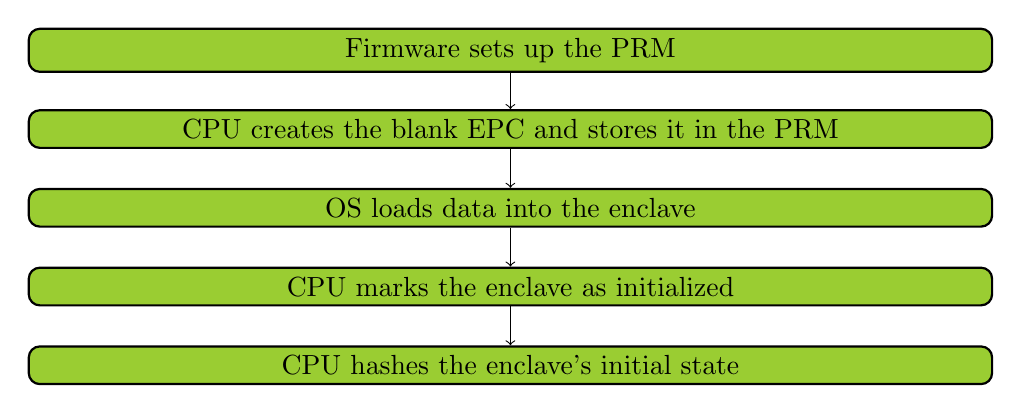
\begin{tikzpicture}[
    block/.style ={rectangle, draw=black, thick, fill=YellowGreen,
          text width=12cm, text centered, rounded corners},
    line/.style ={draw, ->}
]

\node[block] (s1) at (0,0) {Firmware sets up the PRM};
\node[block, below of = s1] (s3) {CPU creates the blank EPC and stores it in the PRM};
\node[block, below of = s3] (s5) {OS loads data into the enclave};
\node[block, below of = s5] (s10) {CPU marks the enclave as initialized};
\node[block, below of = s10] (s15) {CPU hashes the enclave’s initial state};

\path [line] (s1) -- (s3);
\path [line] (s3) -- (s5);
\path [line] (s5) -- (s10);
\path [line] (s10) -- (s15);

\end{tikzpicture}

\caption[Setting Up Intel SGX]{\textbf{Workflow for setting up an enclave.}}
\label{fig:sgx-setup}
\end{figure}

\section{Executing SGX Enclave Code}
Execution flow can only move into an enclave via a special CPU instruction, much like switching from user mode to kernel mode. The actual execution happens in user mode and takes advantage of address translation from the Operating System or hypervisor. The CPU executing the enclave code performs an \gls{aex} whenever execution moves outside the enclave such as servicing an interrupt or during a page fault. The CPU state is saved inside the enclave before exiting ensuring that the CPU can security restore the state of execution. There are special machine mode CPU instructions that are used both in allocating \gls{epc} pages to the enclave as well as evicting those pages into untrusted DRAM. This facilitates code outside the enclave to operate on code within the enclave. \gls{sgx} uses cryptographic protections to assure the confidentiality, integrity and freshness of the evicted \gls{epc} pages while they are stored in untrusted memory \cite{Costan2016}. In this way, Intel \gls{sgx} is able to allow a specific amount of code and data to remain protected while still allowing access to that data by code outside the trust boundary.

\begin{figure}[ht]
\makebox[\textwidth][c]{\begin{tikzpicture}[
	state/.style={draw, ellipse, text width=2cm, minimum height=1.4cm, align=center},
	arrow/.style={-latex'},
	label/.style={text width=3cm, align=center, font=\small}
]
\node[state] (v1) at (0,0) {non-existent};
\node[state] (v2) at (6,0) {not initialized};
\node[state, fill=CornflowerBlue!10!white] (v3) at (6,-4.5) {initialized};
\node[state, fill=CornflowerBlue!10!white] (v4) at (0,-4.5) {initialized\\(in use)};

\draw[arrow]  (v1) edge node[above, label] {ECREATE} (v2);
\draw[arrow]  (v2) edge node[right, label, align=left] {EINIT} (v3);
\draw[arrow]  (v2) edge[loop, looseness=5, in=330, out=30] node[right, label, align=left] {EADD\\EEXTEND} (v2);
\draw[arrow]  (v3) edge[loop, looseness=5, in=300, out=240] node[below, label] {page management instructions} (v3);
\draw[arrow]  (v3) edge[bend left=15] node[below, label] {EENTER\\ERESUME} (v4);
\draw[arrow]  (v4) edge[bend left=15] node[above, label] {EEXIT\\AEX} (v3);
\draw[arrow]  (v3) edge[bend right=15] node[below left, label, align=right, pos=0.7] {EREMOVE} (v1);
\draw[arrow]  (v4) edge[loop, looseness=5, in=300, out=240] node[below, label] {page management instructions} (v4);
\draw[arrow]  (v4) edge[loop, looseness=5, in=210, out=150] node[left, align=right] {EGETKEY\\EREPORT} (v4);
\end{tikzpicture}
}\caption[Intel SGX Enclave Lifecycle]{\textbf{Intel SGX enclave life cycle.} The enclave's memory is protected in states shaded blue. Reprinted as a simplified version from \cite{Costan2016}.\label{figure:sgx-enclave-life-cycle}}
\end{figure}

In order to understand the life cycle of an enclave, we must consider the specific x86 instructions used to create and manage these enclaves. Many of these instructions which create, extend, and remove enclaves operate in ``ring 0'' (most privileged), while attestation, entering, and exiting the enclave can be done in ``ring 3'' (application code). The first of the privileged instructions is ECREATE which fills a protected data structure located inside the \gls{epc} with the size and hash of the enclave. This data structure, called the \gls{secs}, is used by the hardware and is not directly accessible to software. A developer may then add pages to the \gls{epc} with the EADD instruction, and extend the \gls{epc} page measurement with the EEXTEND instruction. The EEXTEND instruction allows for the accumulation of a hash of all the pages in the \gls{epc}. This measurement can be used later for attestation that the enclave has not been tampered with or changed in some way.

It is important to note that in its uninitialized state, none of the enclave code or data is encrypted. For example, any privileged driver running at ``ring 0'' can have access to these data and structures. Enclaves must be initially built on a system that is known to be secure, such that the measurements taken are considered a ``gold standard'' with which to preform attestation on a local or remote machine at some later time. When the EINIT instruction is called, the enclave is considered fully built, the measurement is locked down, and ``ring 3'' (user) applications can now enter the enclave and attest that it is secure. 

EBLOCK, ETRACK, EWB, and ELOAD\footnote{Actually, two load commands, ELDB and ELDU both load into memory a previously evicted page, with ELDB for blocked and ELDU for unblocked. Pages may be blocked when being prepared for eviction. All future accesses to blocked pages will result in a page fault.} are paging instructions run with ``ring 0'' privileges. The goal is to allow the paging of secure pages into and out of main memory while ensuring the confidentiality and integrity of those pages. Information stored inside the \gls{epc} called the \gls{pcmd} keeps track of the identity of the enclave the page belongs to and a pointer to an access rights structure. There is also a \gls{va} which is used to store the version numbers of pages evicted from the \gls{epc}. These versioned and access controlled pages are therefore hardware protected, and any change to the versioning, access rights, or origins of the page will result in a page fault. It is possible to have 2 instances of the same enclave, however pages cannot be swapped between them, and the hashes of these pages will not be the same.

Once an application has asked for ``ring 0'' components to build the enclave and called EENTER to enter the enclave it may begin execution. The hardware is responsible for saving and restoring (ERESUME) the architectural state of execution should any external events like interrupts or exceptions cause execution to leave the enclave (AEX). The EGETKEY and EREPORT instructions operate in user mode (``ring 3'') and seal data based on the key the developer provides. Using these two instructions SGX applications operating in ``ring 3'' are able to preform attestation of the enclave, perhaps the most vital function of any \gls{tee}.

\section{Attestation with Intel SGX}
Software attestation of enclaves is required to ensure the integrity of the enclave. This attestation can happen locally between two enclaves on the same platform or remotely between two different platforms. As previously noted, the measurement of the enclave includes a SHA-256 hash of the enclave's attributes as well as the content, position, and access rights of its pages. This measurement is stored in a register called MRENCLAVE which represents the enclave's \gls{tcb}. The EREPORT instruction is used to generate a signed report of this \gls{tcb} and the EGETKEY instruction then retrieves the key used to validate said report. Local attestation of enclaves can be done using symmetric encryption as the hardware can ensure the integrity of the single key being used to verify the MRENCLAVE value. Remote attestation must be done using asymmetric encryption (both a public and private key) and requires the remote SGX enabled platform to query an Intel attestation server. 